\scanpage{3}
% Reading orientation: the principal diagrams are upright after a 180-degree rotation.
\[
M\subset L\qquad \times\,\unsure{M'U}
\]
\[
A\;-
\]
\diagram{\begin{tikzcd}[column sep=large,row sep=large]
X \arrow[d,dash] & \\
k \arrow[r,dash] & Y
\end{tikzcd}}

\diagram{\begin{tikzcd}[column sep=large,row sep=large]
X' \arrow[r] \arrow[dr,"\unsure{\ne\varnothing}"'] & X \arrow[d,dash]\\
& k
\end{tikzcd}}

\diagram{\begin{tikzcd}[column sep=large,row sep=large,
execute at end picture={
\draw (-1.65,0.1) to[bend left=22] (1.65,0.1);
\draw (-1.8,-0.35) to[bend right=18] (-1.8,-1.75);
}]
\unsure{Y} \arrow[d,"f"] & \unsure{Y'} \arrow[l,"h"'] \arrow[d,"f'"'] & \unsure{V'}\\
X & X' \arrow[l,"g",very thick] &\\
\unsure{g(U')} & \unsure{\supset U'\ne\varnothing} &
\end{tikzcd}}

\diagram{\begin{tikzcd}[column sep=large,row sep=large]
\unsure{Y} \arrow[r] \arrow[dr,dash] & X \arrow[d,dash]\\
& k
\end{tikzcd}}
\diagram{\begin{tikzcd}[column sep=large,row sep=large,
execute at end picture={
\draw (0,-1.3) ellipse (0.35 and 0.24);
\draw (-0.2,-1.4)--(0.2,-1.2);
\draw (-0.1,-1.45)--(0.25,-1.25);
\draw (0.55,-1.05)--(0.55,-2.25);
\draw[->] (0.55,-1.05)--(0.55,-2.25);
}]
Y' \arrow[r] \arrow[dr,dash,bend right=10] & X' \arrow[d,dash]\\
k \arrow[r,dash] & k'
\end{tikzcd}}

\diagram{\begin{tikzcd}[column sep=large,row sep=large,
execute at end picture={
\draw (-1.7,0.25) to[bend left=20] (1.65,0.25);
\draw (-1.6,-0.2) to[bend right=10] (-1.5,-1.65);
\draw (1.3,0.05) to[bend left=8] (1.45,-1.7);
\draw (1.45,0.05) to[bend left=8] (1.6,-1.7);
}]
k' & |[draw,circle]| \unsure{X} \arrow[d] & \unsure{X_K|XK} \arrow[l,very thick] \arrow[d,dash,very thick]\\
& k & K \arrow[l,dash]
\end{tikzcd}}

\figure{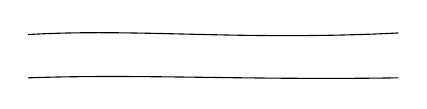
\begin{tikzpicture}
\draw (0,0) .. controls (1.4,0.08) and (2.7,-0.08) .. (4.7,0.02);
\draw (0,-0.55) .. controls (1.4,-0.50) and (2.8,-0.58) .. (4.7,-0.55);
\end{tikzpicture}}
\mspage{2}
